%version of 09-28-18

\chapter{ARITHMETIC}
\label{ch:arithmetic}

**HERE -- SOME INTRO

\section{Arithmetic Operations and Their Laws}
\label{sec:Arithmetic-Tools+Laws}
\index{laws of arithmetic}

Numbers are {\it adjectives}\index{number!as adjective}---you have
five apples and three oranges---but in contrast to adjectives that are
purely descriptive---the red ball, the big dog---numbers can be {\em
  manipulated},\index{number!as {\em manipulable} adjective} using the
tools of {\it arithmetic}.

\subsection{The Tools of Arithmetic}
\label{sec:arithmetic-tools}

The basic tools of arithmetic reside in a small set of operations,
together with two special integers that play important roles with
respect to the operations.  Since these entities are so tightly
intertwined, we discuss them simultaneously.

\smallskip

\noindent {\small\sf Two special integers}
%
The integers zero ($0$)\index{number!zero ($0$)} and one
($1$),\index{number!one ($1$)} play special roles within all four of
the classes of numbers we have described.

\smallskip

\noindent {\small\sf  The operations of arithmetic}\index{arithmetic!basic operations}
%
Arithmetic on the four classes of numbers that we have described is
built upon a rather small repertoire of operations.  When we say that
an operation produces a number ``of the same sort'', we mean that it
produces
\begin{itemize}
\item
an integer result from integer arguments;
\item
a rational (number) result from rational (number) arguments;
\item
a real (number) result from real (number) arguments;
\item
a complex (number) result from complex (number) arguments;
\end{itemize}
The fundamental operations on numbers are, of course, familiar to the
reader.  Our goal in discussing them is to stress the laws that govern
the operations.  Along the way, we also introduce a few operations
that are less familiar but no less important.

\subsubsection{Unary (single-argument) operations}

\addcontentsline{toc}{paragraph}{A. Negating and reciprocating numbers}
\noindent {\small\sf A. Negating and reciprocating numbers.}
\index{arithmetic!basic operations!negation}
%
\noindent {\it i. The operation of {\em negation}}:
\index{arithmetic!basic operations!negating}
\begin{itemize}
\item
is a {\em total function} on the sets $\Z, \Q, \R, \C$.  It replaces
a number $a$ by its {\em negative},
\index{number!negative}
a number of the same sort, denoted $-a$.
\item
is a {\em partial function} on the nonnegative subsets
of $\Z, \Q, \R, \C$.  It replaces a number $a$ by its negative, $-a$,
whenever both $a$ and $-a$ belong to the nonnegative subset being
operated on.
\end{itemize}
Zero ($0$) is the unique {\it fixed point}\index{function!fixed
  point}\index{arithmetic!negation!fixed point} of the operation,
meaning that $0$ is the unique number $a$ such that $a = -a$.

\medskip

\noindent {\it ii. The operation of {\em reciprocation}}:
\index{arithmetic!basic operations!reciprocal}
\begin{itemize}
\item
\index{arithmetic!basic operations!reciprocating}
is a {\em total function} on the sets $\Q, \R, \C$, which replaces each
number $a$ by its {\em reciprocal}, 
\index{number!reciprocal}
a number of the same sort, denoted $1/a$ or $\displaystyle {1 \over
  a}$.  We shall employ whichever notation enhances legibility.

\item
is {\em undefined} on every integer $a$ except for $1$.
\end{itemize}

\medskip

\addcontentsline{toc}{paragraph}{B. Floors, ceilings, magnitudes}
\noindent {\small\sf B. Floors, ceilings, magnitudes.}
\index{arithmetic!basic operations!floor}
\index{arithmetic!basic operations!ceiling}
\index{arithmetic!basic operations!absolute value}
\index{arithmetic!basic operations!magnitude}

\noindent {\it i. The operations of {\em taking floors and ceilings}}
are total operations on the sets $\N, \Z, \Q, \R$.
\begin{itemize}
\item
The {\it floor} of a number $a$, also called {\it the integer part}
\index{arithmetic!basic operations!integer part of a number}
\index{arithmetic!basic operations!floor of a number}
of $a$, denoted $\lfloor a \rfloor$, is the largest integer that does
not exceed $a$; i.e.,:
\[
\lfloor a \rfloor \ \eqdef \ \max_{b \in {\mathbb{N}}} \Big[ b \ \leq a \Big]
\]
\item
The {\it ceiling} of a number $a$
\index{arithmetic!basic operations!ceiling of a number}
of $a$, denoted $\lceil a \rceil$, is the smallest integer that is 
not smaller than $a$:
\[
\lceil a \rceil \ \eqdef \ \min_{b \in {\mathbb{N}}} \Big[ b \ \geq a \Big]
\]
\end{itemize}
Thus, the operations of taking floors and ceilings are two ways to
{\em round} rationals and reals to their ``closest''
integers.\index{arithmetic!basic operations!rounding to ``closest'' integer}

\medskip

\noindent {\it ii. The operations of taking {\em absolute values/magnitudes}}:
\index{arithmetic!basic operations!absolute value, magnitude}
%
Let $a$ be a real number.  The {\it absolute value}, or, {\it
  magnitude}, of $a$, denoted $|a|$ equals either $a$ or $-a$,
whichever is positive.  For a complex number $a$, the definition of
$|a|$ is more complicated: it is a measure of $a$'s ``distance'' from
the ``origin'' complex number $0 + 0 \cdot i$.  In detail:
\[
|a| \ = \ \left\{
\begin{array}{cl}
a & \mbox{ if } \ [a \in \R] \ \ \mbox{ and } [a \geq 0] \\
-a & \mbox{ if } \ [a \in \R] \ \ \mbox{ and } [a < 0] \\
\sqrt{b^2 + c^2} &  \mbox{ if } \ [a \in \C]  \ \ \mbox{ and } [a = (b+ci)]
\end{array}
\right.
\]

\medskip

\addcontentsline{toc}{paragraph}{C. Factorials (of nonnegative integers)}
\noindent {\small\sf C. Factorials (of nonnegative integers).}
\index{arithmetic!basic operations!factorial (of a nonnegative integer)}
%
The {\it factorial} of a nonnegative integer $n \in \N$, which is
commonly denoted $n!$,
\index{arithmetic!basic operations!$n!$: factorial of $n \in \N$}
\index{arithmetic!basic operations!factorial of nonnegative integer}
is the function defined via the following recursion.
\begin{equation}
\label{eq:n-factorial-recursion}
\mbox{\sc fact}(n) \ = \ \left\{
\begin{array}{cl}
1 & \mbox{  if } \ n=0 \\
n \cdot \mbox{\sc fact}(n-1) & \mbox{  if } \ n>0
\end{array}
\right.
\end{equation}
By ``unwinding'' the recursion in (\ref{eq:n-factorial-recursion}),
one finds that, for all $n \in \N$,
\begin{equation}
\label{eq:n-factorial-direct}
n! \ = \ \mbox{\sc fact}(n) \ = \ 
n \cdot (n-1) \cdot (n-2) \cdot \cdots \cdot 2 \cdot 1
\end{equation} 
A $3$-step inductive argument validates this ``unwinding'':
\begin{enumerate}
\item
If $n =0$, then {\sc fact}$(n) = 1$, by definition
(\ref{eq:n-factorial-recursion}).
\item
Assume, for induction, that the expansion in
(\ref{eq:n-factorial-direct}) is valid for a given $k \in N$:
\[ \mbox{\sc fact}(k) \ = \ k \cdot (k-1) \cdot (k-2) \cdot \cdots
\cdot 2 \cdot 1 \] 
\item
Then:
\[
\begin{array}{lclll}
\mbox{\sc fact}(k+1) & = & (k+1) \cdot \mbox{\sc fact}(k)
  & & \mbox{by (\ref{eq:n-factorial-recursion})} \\
  & = &
(k+1) \cdot k \cdot (k-1) \cdot (k-2) \cdot \cdots \cdot 2 \cdot 1
  & & \mbox{by induction}
\end{array}
\]
\end{enumerate}


\subsubsection{Binary (two-argument) operations}
\label{sec:binary-operators}

\paragraph{\small\sf A. Addition and Subtraction.}
\index{arithmetic!basic operations!addition}
\index{arithmetic!basic operations!subtraction}
%
The operation of {\it addition}\index{arithmetic!addition} is a {\em
  total function} that replaces any two numbers $a$ and $b$ by a
number of the same sort.  The resulting number is the {\em sum of $a$
  and $b$}\index{arithmetic!addition!sum} and is denoted $a+b$.

\noindent
The operation of {\it subtraction}\index{arithmetic!subtraction} is a
{\em total function} on the sets $\Z, \Q, \R, \C$, which replaces any
two numbers $a$ and $b$ by a number of the same sort.  The resulting
number is the {\em difference of $a$ and $b$}
\index{arithmetic!subtraction!difference} and is denoted $a-b$.  On
the nonnegative subsets of the sets $\Z, \Q, \R, \C$---such as $\N$,
which is the largest nonnegative subset of $\Z$---subtraction is a
{\em partial function}, which is defined only when $a \geq b$.

Subtraction can also be defined as follows.  For any two numbers $a$
and $b$, {\em the difference of $a$ and $b$ is the sum of $a$ and the
  negation of $b$}; i.e.,
\[ a-b \ = \ a + (-b) \]

{\em The special role of $0$ under addition and subtraction.}
%
The number $0$ is the {\it identity} under addition and
  subtraction.\index{number!additive identity}\index{number!identity
  under addition}\index{identity!additive}
%
This means that, for all numbers $a$,
\[ a+0 \ = \ a-0 \ = \ a. \]

{\em The special role of $1$ under addition and subtraction.}
%
For any integer $a$, there is no integer between $a$ and $a+1$ or
between $a-1$ and $a$.  For this reason, on the sets $\Z$ and $\N$,
one often singles out the following special cases of addition and
subtraction, especially in reasoning about situations that are indexed
by integers.  Strangely, these operations have no universally accepted
notations.
\begin{itemize}
\item
The {\it successor} operation\index{arithmetic!integers!successor} is
a {\em total function} on both $\N$ and $\Z$, which replaces an
integer $a$ by the integer $a+1$.
\item
The {\it predecessor} operation\index{arithmetic!integers!predecessor}
is a {\em total function} on $\Z$, which replaces an integer $a$ by
the integer $a-1$.  It is a {\em partial function} on $\N$, which is
defined only when the argument $a$ is positive (so that $a-1 \in \N$).
\end{itemize}

The operations of addition and subtraction are said to be {\em
  mutually inverse operations}\index{arithmetic!integers!additive
  inverse} \index{arithmetic!integers!addition and subtraction are
  mutually inverse} of each other because each can be used to ``undo''
the other:
\[
a \ = \ (a+b) -b \ = \ (a-b) +b
\]

\medskip

\addcontentsline{toc}{paragraph}{B. Multiplication and Division}
\noindent {\small\sf B. Multiplication and Division}.
\index{arithmetic!basic operations!multiplication}
\index{arithmetic!basic operations!division}
%
The operation of {\it multiplication}\index{arithmetic!multiplication}
is a {\em total function} that replaces any two numbers $a$ and $b$ by
a number of the same sort.  The resulting number is the {\em product
  of $a$ and $b$}\index{arithmetic!multiplication!product} and is
denoted either $a \cdot b$ \index{arithmetic!multiplication!$a \cdot  b$}
or $a \times b$.\index{arithmetic!multiplication!$a \times b$}
We shall usually favor the former notation, except when the latter
enhances legibility.

The operation of {\it division}\index{arithmetic!division} is a {\em
  partial function} on all of our sets of numbers.  Given two numbers
$a$ and $b$, the result of dividing $a$ by $b$---{\em when that result
  is defined}---is the {\it quotient of $a$ by $b$}
\index{arithmetic!division!When is $a/b$ defined?}
\index{arithmetic!division!quotient}
\index{arithmetic!division!quotient!$a/b$}
\index{arithmetic!division!quotient!$a \div b$}
\index{arithmetic!division!quotient!${a \over b}$}
and is denoted by one of the following three notations: $a/b$, $a \div
b$, $\displaystyle{a \over b}$.  The {\it quotient of $a$ by $b$} is
defined precisely when {\em both}

\noindent
\hspace*{.35in}(1) $b \neq 0$: one can never divide by $0$ \\
\hspace*{.35in}{\em and} \\
\hspace*{.35in}(2) there exists a number $c$ such that $a = b \cdot c$.

\noindent
Assuming that condition (1) holds, {\em condition (2) always holds
  when $a$ and $b$ belong to $\Q$ or $\R$ or $\C$}.

Division can also be defined as follows.  For any two numbers $a$
and $b$, {\em the quotient of $a$ and $b$ is the product of $a$ and the
reciprocal of $b$} (assuming that the latter exists); i.e.,
\[ a/b \ = \ a \cdot (1/b). \]
Computing reciprocals of nonzero numbers in $\Q$ and $\R$ is standard
high-school level fare; computing reciprocals of nonzero numbers in
$\C$ requires a bit of calculational algebra which we do not cover.
For completeness, we note that the reciprocal of the {\em nonzero}
complex number $a + bi \in \C$ is the complex number $c+di$ where
\[ c \ = \ \frac{a}{a^2 + b^2} \ \ \ \ \
\mbox{ and } \ \ \ \ \
d \ = \ \frac{-b}{a^2 + b^2}.
\]

{\em The special role of $1$ under multiplication and division.}
%
The number $1$ is the {\it identity} under the operations of
multiplication and division.\index{number!multiplicative
  identity}\index{number!identity under
  multiplication}\index{identity!multiplicative}
%
This means that, for all numbers $a$,
\[ a \cdot 1 \ = \ a \cdot (1/1) \ = \ a. \]

{\em The special role of $0$ under multiplication and division.}
%
The number $0$ is the {\it annihilator} under
multiplication.\index{multiplicative annihilator} This means that, for
all numbers $a$
\[ a \cdot 0 \ = \ 0. \]

The operations of multiplication and division are said to be {\em
  inverse operations}\index{arithmetic!integers!multiplicative
  inverse} \index{arithmetic!integers!multiplication and division are
  mutually inverse} because, when both operations can be applied, each
can be used to ``undo'' the other:
\[ a = (a \cdot b) \div b \ = \ (a \div b) \cdot b.  \]

\medskip

%\addcontentsline{toc}{paragraph}{C. Binomial coefficients and Pascal's triangle}
\paragraph{\small\sf C. Binomial coefficients and Pascal's triangle}
\index{arithmetic!basic operations!binomial coefficient}

We close our catalogue of arithmetic operations with a binary
operation on\footnote{In advanced contexts, one encounters binomial
  coefficients with non-integer arguments.}~$\N \times \N$.

Let $n$ and $k \leq n$ be nonnegative integers (i.e., elements of
$\N$).  The {\it binomial coefficient} denoted either as
$\displaystyle {n \choose k}$ or as $\Delta_{n,k}$, is the number
\index{binomial coefficients}
\begin{equation}
\label{eq:binom-coeff}
\Delta_{n,k} \ = \
{n \choose k} \ \eqdef \ \frac{n!}{k!(n-k)!} \ = \
\frac{n(n-1)(n-2) \cdots (n-k+1)}{k (k-1)(k-2) \cdots 1}
\end{equation}
Many of the secrets of these wonderful numbers---including the fact
that they are {\em integers}---can be deduced from the following
results.

\begin{prop}
\label{thm:manipulate-binom-coeff}
For all $n, k \in \N$ with $k \leq n$:

{\rm (a)} The symmetry rule:
\index{binomial coefficients!symmetry rule}
\begin{equation}
\label{eq:symmetry-binom-coeff}
{n \choose k} \ = \ {n \choose {n-k}}
\end{equation}

{\rm (b)} The addition rule:
\index{binomial coefficients!addition rule}
\begin{equation}
\label{eq:add-binom-coeff}
{n \choose k} \ + \ {n \choose {k+1}} \ = \ {{n+1} \choose {k+1}}
\end{equation}
\end{prop}

\begin{proof}
($a$)
We verify equation (\ref{eq:symmetry-binom-coeff}) by
(\ref{eq:binom-coeff}) plus the commutativity of multiplication (see
Section~\ref{sec:Arithmetic-Laws}),
\begin{eqnarray*}
{n \choose k} & = & \frac{n!}{k!(n-k)!} \\
              & = & \frac{n!}{(n-k)!k!} \\
              & = & {n \choose {n-k}}
\end{eqnarray*}

\noindent ($b$)
We verify equation (\ref{eq:add-binom-coeff}) by explicitly adding the
fractions exposed by (\ref{eq:binom-coeff}):
\begin{eqnarray*}
{n \choose k} \ + \ {n \choose {k+1}}
  & = &
\frac{n!}{k!(n-k)!} \ + \ \frac{n!}{(k+1)!(n-k-1)!} \\
  & = &
n! \cdot \frac{(k+1) + (n-k)} {(k+1)!(n-k)!} \\
  & = & 
\frac{(n+1)!}{(k+1)!(n-k)!} \\
  & = &
{{n+1} \choose {k+1}} \hspace*{2in} \qed
\end{eqnarray*}

Extrapolating from Proposition~\ref{thm:manipulate-binom-coeff}, we now
present {\it Pascal's triangle}, named in honor of
\index{Pascal's triangle}
\index{Pascal, Blaise}
the French polymath Blaise Pascal.  Fig.~\ref{fig:pascal-triangle}
provides a ``prefix'' of this famed array of integers, for $n,k \leq
5$.
\begin{figure}[htb]
\[
\begin{array}{c||r|r|r|r|r|r|r}
{\displaystyle {n \choose k}} & k=0 & k=1 & k=2 & k=3 & k=4 & k=5 &\ldots \\
\hline
\hline
n=1 & 1 & 1 &    &    &    &   & \ldots \\
\hline
n=2 & 1 & 2 & 1  &    &    &   & \ldots \\
\hline
n=3 & 1 & 3 & 3  & 1  &    &   & \ldots \\
\hline
n=4 & 1 & 4 & 6  & 4  & 1  &   & \ldots \\
\hline
n=5 & 1 & 5 & 10 & 10 & 5  & 1 & \ldots \\
\hline
\vdots &\vdots &\vdots &\vdots &\vdots &\vdots &\vdots &\ddots
\end{array}
\]
\caption{A ``prefix'' of Pascal's Triangle, for $n,k \leq 5$.}
\label{fig:pascal-triangle}
\end{figure}
The formation rule of the array is:
\begin{description}
\item[\sf Formation rule for Pascal's triangle:]
% 
{\it The entry at (row $n+1$, column $k+1$) is the sum of the entries
  at (row $n$, column $k$) and (row $n$, column $k+1$).}
\end{description}
\qed
\end{proof}


If you compare the formation rule for Pascal's triangle with equation
(\ref{eq:add-binom-coeff}), then you may anticipate the following
result.

\addcontentsline{toc}{paragraph}{-- A fun result: Pascal's triangle
  and the binomial coefficients}

\begin{prop}
\label{thm:pascal-binom}
The entries of Pascal's triangle are the binomial coefficients.
Specifically, for all $n,k$, the entry at (row $n$, column $k$) of the
Triangle is $\displaystyle {n \choose k}$.
\end{prop}

\begin{proof}
We note by observation and direct calcullation (see
Fig.~\ref{fig:pascal-triangle}) that the proposition is true for $n =
1$ and $k \in \{0, 1\}$.  A simple double induction

\noindent
****************** \\
induction on $n$, then for each value of $n$ on $k \leq n$ \\
{\Arny SHOULD WE SPELL THIS OUT IN DETAIL?  GIVE AS AN EXERCISE?} \\
******************

\noindent
verifies that every binomial coefficient appears in the Triangle and
every Triangle entry is a binomial coefficient.  \qed
\end{proof}

\medskip

\addcontentsline{toc}{paragraph}{-- A fun result: Binomial
  coefficients are integers}

\begin{prop}
\label{thm:binomcoeff-integer}
Every binomial coefficient is an integer.
\end{prop}

\begin{proof}
Since every entry in Pascal's triangle is obtained from integers via
repeated additions, this result follows from
Proposition~\ref{thm:pascal-binom}.  \qed
\end{proof}

\bigskip

Binomial coefficients are indispensable when studying myriad topics
related to {\em counting}, such as:
\begin{itemize}
\item
what are the relative likelihoods of various $5$-card deals from a
fair $52$-card deck?
\item
What is the likelihood of observing $15$ {\sc head}s and $25$ {\sc
  tail}s in $40$ flips of a fair coin?
\item
What are the comparative operation-count costs of Merge-Sort and
Quick-Sort when sorting $n$ keys; cf.~\cite{CLRS}?

\end{itemize}
We shall, therefore, see a lot more about binomial coefficients in
Section~\ref{sec:powers+polynolmials} and Chapter~\ref{ch:prob-stat}.
With each subsequent encounter, our respect for these numbers will
grow.


\subsection{The Laws of Arithmetic, and applications}
\label{sec:Arithmetic-Laws}
\index{arithmetic!basic laws}

The student should understand the following laws of arithmetic on the
reals, rationals, and reals---and be able to employ them cogently in
rigorous argumentation.


\paragraph{\small\sf A. The commutative law.}
\index{commutative law!arithmetic}
\index{commutative law!addition}
\index{commutative law!multiplication}
\index{arithmetic!commutative law}

For all numbers $x$ and $y$:
\[
\begin{array}{llc}
\mbox{\it for addition:}
  & & x+y \ = \ y+x \\
\mbox{\it for multiplication:}
  & & x \cdot y \ = \ y \cdot x
\end{array}
\]


\paragraph{\small\sf B. The associative law}
\index{associative law for arithmetic}
\index{arithmetic!associative law}

For all numbers $x$, $y$, and $z$,
\[ (x+y)+z \ = \ x+(y+z) \ \ \ \mbox{\bf and } \ \ 
x\cdot (y\cdot z) 
(x \cdot y) \cdot z \ = \ x\cdot (y\cdot z). \] 
This allows one, for instance, to write strings of additions or of
multiplications without using parentheses for grouping.


\paragraph{\small\sf C. The distributive law}
\index{distributive law for arithmetic}
\index{arithmetic!distributive law}

For all numbers $x$, $y$, and $z$,
\begin{equation}
\label{eq:distr-law}
x \cdot (y + z) \ = \ (x \cdot y) + (x \cdot z).
\end{equation}
One commonly articulates this law as, ``{\em Multiplication
  distributes over addition.}''


One of the most common uses of the distributive law reads equation
(\ref{eq:distr-law}) ``backwards,'' thereby deriving a formula for
{\em factoring} \index{arithmetic!factoring} complex expressions that
use both addition and multiplication.

Easily, addition does {\em not} distribute over multiplication; i.e.,
in general, $x + y \cdot z \ \neq \ (x+y) \cdot (x+z)$.  Hence, when
we see ``$x + y \cdot z$'', we know that the multiplication is
performed before the addition.  In other words, {\em Multiplication
  takes priority over addition.}  \index{arithmetic!priority of
  multiplication over addition} This priority permits us to write the
righthand side of (\ref{eq:distr-law}) without parentheses, as in
\[ x \cdot (y + z) \ = \ x \cdot y + x \cdot z. \]

Via multiple invocations of the preceding laws, we can derive a recipe
for multiplying complicated expressions.  We illustrate this via the
``simplest'' complicated expression, $(a+b) \cdot (c+d)$.

\begin{prop}
\label{prop:(a+b)(c+d)}
For all numbers $a, b, c, d$:
\begin{equation}
\label{eq:(a+b)(c+d)}
(a+b) \cdot (c+d) \ = \ a \cdot c + a \cdot d + b \cdot c + b \cdot d
\end{equation}
\end{prop}

\begin{proof}
Note first that because multiplication takes priority over addition,
the absence of parentheses in expressions such as
(\ref{prop:(a+b)(c+d)}) does not jeopardize unambiguity.  Our proof of
the proposition invokes the laws we have just enunciated multiple
times.
\[
\begin{array}{lclll}
(a+b) \cdot (c+d) & = & (a+b) \cdot c \ + \ (a+b) \cdot d
& & \mbox{distributive law} \\ 
  & = & c \cdot (a+b) \ + \ d \cdot (a+b)
& & \mbox{commutativity of multiplication} \ (2 \times) \\
  & = & c \cdot a + c \cdot b + d \cdot a + d \cdot b 
& & \mbox{distributive law} \ (2 \times) \\
  & = & a \cdot c + b \cdot c + a \cdot d + b \cdot d
& & \mbox{commutativity of multiplication} \ (4 \times) \\
  & = &  a \cdot c + a \cdot d + b \cdot c + b \cdot d
& & \mbox{commutativity of addition}
\end{array}
\]
\qed
\end{proof}


We close our short survey of the laws of arithmetic with the following
important two-part law.
\begin{itemize}
\item
{\it The law of inverses}.\index{inverse laws for
  arithmetic}\index{laws of arithmetic!inverse laws}
%
  \begin{itemize}
  \item
Every number $x$ has an {\em additive inverse},\index{additive inverse}
i.e., a number $y$ such that $x+y =0$.  This inverse is $x$'s {\it
  negative} $-x$.\index{additive inverse!negative as additive inverse}
  \item
Every {\em nonzero} number $x \neq 0$ has a {\em multiplicative
  inverse},\index{multiplicative inverse} i.e., a number $y$ such that
$x \cdot y = 1$.  This inverse is $x$'s {\it reciprocal},
$1/x$.\index{multiplicative inverse!reciprocal as multiplicative inverse}
  \end{itemize}
\end{itemize}

We close this section with another of our ``fun'' propositions.

\addcontentsline{toc}{paragraph}{-- A fun result: A ``trick'' for
  squaring some integers}

\begin{prop}
\label{thm:75x65=4925}
Let $n$ be any number that has a $2$-digit decimal of the form $\delta
5$, where $\delta \in \{ 0,1,2,3,4,5,6,7,8,9 \}$,
so that
\[ n \ = \ 10 \cdot \delta + 5
\]
Then 
\[ n^2 \ = \ 100 \cdot \delta \cdot (\delta+1) + 25. \]
In other words, one obtains a base-$10$ numeral for $n^2$ by
multiplying $\delta$ by $\delta +1$ and appending $25$ to the product.
\end{prop}

\noindent
Examples of Proposition ~\ref{thm:75x65=4925} include
$25^2 = 625$ (because $2 \cdot 3 = 6$) and $75^2 = 5625$ (because $7
\cdot 8 = 56$).

\begin{proof} (for general $\delta$).
%
We invoke Proposition~\ref{prop:(a+b)(c+d)} and the distributive law.
\[
\begin{array}{lclll}
n^2 & = & (10 \cdot \delta + 5)^2 & & \mbox{Given} \\
    & = & 100 \cdot \delta^2 \ + \ 100 \cdot delta \ + \ 25
              & & \mbox{the proposition} \\
    & = & 100 \cdot (\delta^2 \ + \ \delta) \ + \ 25
              & & \mbox{factoring: distributive law} \\
    & = & 100 \cdot \delta \cdot (\delta + 1) \ + \ 25
              & & \mbox{factoring: distributive law} \\
\end{array}
\]
\qed
\end{proof}


\subsection{Rational Arithmetic: A Worthwhile Exercise}
\label{sec:Rational-arithmetic}
\index{number!rational!arithmetic}

In Section~\ref{sec:rationals} we defined the rational numbers and
reviewed why they were needed to compensate for the general lack of
multiplicative inverses in the integers.  But we did not review how to
perform arithmetic on the elements of the set $\Q$.  We correct this
shortcoming now.  Of course, the reader will have encountered rational
arithmetic long ago---but we are now reviewing the topic in order to
provide the reader with a set of worthwhile exercise to reinforce the
mathematical thinking whose presentation is our main goal.

\medskip

The rational numbers build their rules for arithmetic upon the
corresponding rules for integers.  For all $p/q$ and $r/s$ in $\Q$:
\[
\begin{array}{|llcl|}
\hline
\mbox{\small\sf Addition:} & 
{\displaystyle
{p \over q} + {r \over s} }
  & = &
{\displaystyle
 \frac{p \cdot s + r \cdot q}{q \cdot s} }  \\
 & & & \\
\mbox{\small\sf Subtraction:} &
{\displaystyle
{p \over q} + {r \over s} }
  & = & 
{\displaystyle
{p \over q} + {(-r) \over s} } \\
 & & & \\
\mbox{\small\sf Multiplication:} &
{\displaystyle
{p \over q} \cdot {r \over s} }
  & = & 
{\displaystyle
\frac{p \cdot r}{r \cdot s} } \\
  & & & \\
\mbox{\small\sf Division:} &
{\displaystyle
{p \over q} \div {r \over s} }
  & = &
{\displaystyle
{p \over q} \cdot {s \over r} } \\
\hline
\end{array}
\]

It is worth verifying that rational arithmetic as thus defined behaves
in the required manner; in particular that rational arithmetic:
\begin{itemize}
\item
works correctly when the argument rational numbers are, in fact,
integers, i.e., when $q = s = 1$ in the preceding table.
\item
treats the number $0$ appropriately, i.e., as an additive identity and
a multiplicative annihilator; cf., Sections~\ref{sec:arithmetic-tools}
and~\ref{sec:Arithmetic-Laws}.
\item
obeys the required laws; cf., Section~\ref{sec:Arithmetic-Laws}.

Verifying the distributivity of rational multiplication over rational
addition will be a particularly valuable exercise because of the
required amount of manipulation.
\end{itemize}

\section{Basic Algebraic Concepts and Their Manipulations}

\subsection{Powers and polynomials}
\label{sec:powers+polynolmials}

\subsubsection{Raising a number to a power.}
\label{sec:x-toa-power}
A conceptually powerful notational construct is the operation of {\it
  raising a number to a power:}\index{raising a number to a power}
%
For real numbers $a$ and $b$, the {\it $b$th power} of $a$, denoted
$a^b$ is defined by the system of equations
\begin{equation}
\label{eq:power-def}
\begin{array}{llll}
\mbox{for all numbers $a>0$} & & & a^0 = 1 \\
 & & & \\
\mbox{for all numbers $a, b, c$} & & & a^b \cdot a^c = a^{b+c}.
\end{array}
\end{equation}
This deceptively simple definition has myriad consequences which we
often take for granted.
\begin{itemize}
\item
For all numbers $a>0$, the number $a^0 = 1$.

This follows (via cancellation) from (\ref{eq:power-def}) via the fact
that
\[ a^b \cdot a^0 \ = \ a^{b+0} \ = \ a^b \ = \ a^b \cdot 1.  \]

\item
For all numbers $a >0$, the number $a^{1/2}$\index{$a^{1/2}$: the
  square root of number $a$}
is the {\it square root} of $a$,\index{square root}
i.e., $a^{1/2}$ is the (unique, via cancellation) number $b$ such that
$b^2 = a$.  Another common notation for The number $a^{1/2}$ is
$\sqrt{a}$.\index{$\sqrt{a}$: the square root of number $a$}

This follows from (\ref{eq:power-def}) via the fact that
\[ a \ = \ a^1 \ = \ a^{(1/2) + (1/2)} \ = \ a^{1/2} \cdot a^{1/2} \ = \
\left(a^{1/2}\right)^2. \]

\item
For all numbers $a>0$ and $b$, the number $a^{-b}$ is the {\it
  multiplicative inverse}\index{multiplicative inverse}
of $a^b$, meaning that $a^b \cdot a^{-b} = 1$

This follows from (\ref{eq:power-def}) via the fact that
\[ a^b \cdot a^{-b} \ = \ a^{(b + (-b))} \ = \ a^0 \ = \  1 \]
\end{itemize}
When the power $b$ is a positive integer, then definition
(\ref{eq:power-def}) can be cast in the following attractive inductive
form:
\begin{equation}
\label{eq:power-def-integer}
\begin{array}{llll}
\mbox{for all numbers $a>0$} & & & a^0 = 1 \\
 & & & \\
\mbox{for all numbers $a$ and integers $b$} & & & a^{b+1} = a \cdot
a^b.
\end{array}
\end{equation}
Summing up, we now know about powers that are integral or fractional,
positive, zero, or negative


\section{Polynomials and Their Roots}
\label{sec:poly-roots}

We want students to master the notions of polynomials and their
associated notions, such as degrees and coefficients, and computations
therewith, including polynomial summation and multiplication.  While
polynomial multiplication is often considered ``non-elementary'', it
must be mastered in order to fully understand positional number
systems; it is also essential, e.g., when discussing a range of topics
relating to, say, fault tolerance and encryption).

**DEFINE ``degree''

\subsection{Univariate Polynomials}
\label{sec:univariate-polynomials}
\index{polynomials!univariate}


\subsubsection{Degree-$d$ univariate polynomials have $d$ roots}
\label{sec:fund-thm-algebra}

\index{The Fundamental Theorem of Algebra}
\begin{theorem}[The Fundamental Theorem of Algebra]
Every degree-$d$ univariate polynolmial with complex coefficients has
$d$ complex roots 
\end{theorem}

\subsection{Finding the Roots of Univariate Polynomials}

\subsubsection{Milestones in the quest for roots}

Al-Khwarizmi,
Descartes

\subsubsection{Solving quadratic univariate polynomials}

** quadratic means degree-$2$

\paragraph{\small\sf A. A special case with an interesting solution}

Al-Khwarizmi

{\ignore {\Denis It is interesting here to stress how hard it was to solve such equations. Algebra raised only in the second half of the last millenium.
However, there are several nice examples of geometrical solutions.
One of the oldest comes from babylonians in the 18th century BC.
The numeral system was in base 60, and the problem was to determine the length of the side of a square which was part of a larger rectangle.
The following figure details the process.}}
{\Denis Add here a small introduction about solving polynomial of degree 2 from El Kwharizmi, or remove it and put it as an exercice.}
\begin{figure}[htb]
\begin{center}
       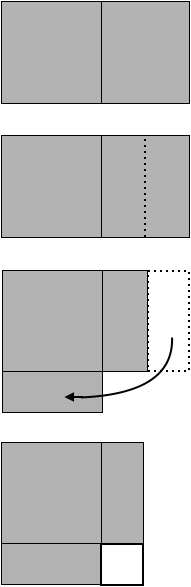
\includegraphics[scale=0.4]{FiguresArithmetic/tabletteMesopotamie}
\caption{Solving $x^2 + x = 45$.
The idea of the proof is to represent the left hand side by the square $x^2$ beside a rectangle $60 \times x$.
Then, split the right rectangle into two equal parts and move one part a the bottom of the left square.
The final figure shows the whole square whose surface is equal to $45$ plus the surface of the white square
whose surface is equal to $30 \times 30$.
In base $60$, this is $15$. 
$45+15 = 60$, thus, the big square is the unit square, its side is $60$.
Thus, the length of the initial square is equal to $60-30=30$.}
\label{fig:equationBabillon}
\end{center}
\end{figure}



\paragraph{\small\sf B. The technique of ``completing the square''}

\paragraph{\small\sf C. Specifying the roots of a quadratic univariate polynomial}


\subsection{Bivariate Polynomials}
\label{sec:bivariate-polynomials}
\index{polynomials!bivariate}



\index{The Binomial Theorem}
\subsubsection{The Binomial Theorem.}
\label{sec:Binomial-thm}

Perhaps the simplest bivariate polynomials are the ones in the
following family.
\begin{equation}
\label{eq:binomial-polys}
\mbox{For } \ n \in \N^+, \hspace*{.5in}
P_n(x,y) \ \eqdef \ (x+y)^n.
\end{equation}
There are lessons to be learned from the structure of these
polynomials, so let us begin to expand them using the arithmetic
techniques we have learned earlier.
\begin{eqnarray*}
P_1(x,y) \ = \
(x+y)^1 & = & x+y  \\
P_2(x,y) \ = \
(x+y)^2 & = & (x+y) \cdot (x+y) \\
        & = & x^2 + 2xy + y^2 \\
P_3(x,y) \ = \
(x+y)^3 & = & (x+y) \cdot (x^2 + 2xy + y^2) \\
   & = & (x^3 + 2x^2y +  xy^2) + (x^2y + 2xy^2 + y^3) \\
   & = & x^3 + 3x^2y + 3xy^2 + y^3  
\end{eqnarray*}

Let us stop to review what we are seeing.  We have remarked before
that doing mathematics can sometimes involve a wonderfully exciting
(quite sophisticated) pattern-matching game.  So, let us pattern-match!
\begin{enumerate}
\item
The coefficients of the expanded $P_1(x,y)$ are $\langle 1,1 \rangle$.
\item
The coefficients of the expanded $P_2(x,y)$ are $\langle 1,2,1 \rangle$.
\item
The coefficients of the expanded $P_3(x,y)$ are $\langle 1,3,3,1 \rangle$.
\end{enumerate}
There is a pattern emerging here.  Can you spot it?  Where have we
seen a pattern of tuples that begins in the same manner?  As a rather
broad hint, look at Fig.~\ref{fig:pascal-triangle}!  Could the
coefficients of each $P_n$ possibly be the successive binomial
coefficients
\[ {n \choose 0}, \ {n \choose 1}, \ \ldots, \ {n \choose {n-1}}, \ {n
  \choose n}
\]
Let us use induction to explore this possibility by expanding a
generic $P_n$ with symbolic ``dummy'' coefficients and see what this
says about $P_{n+1}$.  To this end, let $a_{n,n-r}$ denote the
coefficient of $x^{n-r} y^r$ in the expansion of $P_n(x,y)$.  Using
our ``dummy'' coefficients, we have
\[ 
\begin{array}{l}
P_n(x,y) \ = \
 x^n \ + \ \cdots \ + \ a_{n,n-r} x^{n-r} y^r
    \ + \ a_{n,n-r-1} x^{n-r-1} y^{r+1} \\
\hspace*{1in} + \ a_{n,n-r-2} x^{n-r-2} y^{r+2}
 \ + \ \cdots \ + \ y^n
\end{array}
\]
Continuing with this symbolic evaluation, we have:
\begin{equation}
\label{eq:xPk}
\begin{array}{l}
x \cdot P_n(x,y) \ = \
 x^{n+1} \ + \ \cdots \ + \ a_{n,n-r} x^{n-r+1} y^r
    \ + \ a_{n,n-r-1} x^{n-r} y^{r+1} \\
\hspace*{1in} + \ a_{n,n-r-2} x^{n-r-1} y^{r+2}
 \ + \ \cdots \ + \ xy^n
\end{array}
\end{equation}
and
\begin{equation}
\label{eq:yPk}
\begin{array}{l}
y \cdot P_n(x,y) \ = \
 x^n y \ + \ \cdots \ + \ a_{n,n-r} x^{n-r} y^{r+1}
    \ + \ a_{n,n-r-1} x^{n-r-1} y^{r+2} \\
\hspace*{1in} + \ a_{n,n-r-2} x^{n-r-2} y^{r+3}
 \ + \ \cdots \ + \ y^{n+1}
\end{array}
\end{equation}
Because
\[ P_{n+1}(x+y) \ = \ (x+y) \cdot P_n(x,y)
                \ = \ x \cdot P_n(x,y) \ + \ y \cdot P_n(x,y),
\]
the ``dummy'' coefficient $a_{n-r+1,r}$ of $x^{n-r+1} y^r$ in
$P_{n+1}(x+y)$ is the sum of the following coefficients in $P_n(x,y)$:
\begin{center}
$\bullet$
the coefficient $a_{n,n-r}$ of $x^{n-r}y^r$ \ \ \ \ \
and \ \ \ \ \
$\bullet$
the coefficient $a_{n,n-r+1}$ of $x^{n-r+1}y^{r-1}$
\end{center}
By induction, then, for all $n,r \in \N$ with $r \leq n$,
\[ a_{n,r} + a_{n,r+1} \ = \ a_{n+1,r+1} \]
Combining this equation with the observed initial conditions
\[ a_{1,0} \ = \ a_{1,1} \ = \ 1 \]
we see that each coefficient $a_{n,r}$ is actually the binomial
coefficient $\displaystyle {n \choose r}$.  This observation is
attributed to the renowned English mathematician/physicist Isaac
Newton and is enshrined in Newton's famous {\it Binomial Theorem}.

\ignore{**********
so that, finally,
\begin{eqnarray*}
             & = &
 x^{k+1} \ + \ (k+1) x^k y \ + \ \cdots \ + \
   (a_{k,k-r-1} + a_{k,k-r}) x^{k-r} y^{r+1} \\
             &   & \ \ \ + \
   (a_{k,k-r-2} + a_{k,k-r-1}) x^{k-r-1} y^{r+2}
 \ + \ \cdots \ + \ (k+1) xy^k \ + \ y^{k+1} \\
      & = &
 x^{k+1} \ + \ (k+1) x^k y \ + \ \cdots \ + \
 a_{k+1,k-r} x^{k-r} y^{r+1} \\
            &    & \ \ \ + \  a_{k+1,k-r-1} x^{k-r-1} y^{r+2}
 \ + \ \cdots \ + \ (k+1) xy^k \ + \ y^{k+1}
\end{eqnarray*}
*******}

\begin{theorem}[The Binomial Theorem]
\label{thm:Binomial-theorem}
For all $n \in \N$,
\[
(x+y)^n \ = \
\sum_{i=0}^n \ \ {n \choose i} x^{n-i} y^i.
\]
\end{theorem}
\index{The Binomial Theorem!binomial coefficients}
\index{binomial coefficients!The Binomial Theorem}
\index{polynomials!bivariate!The Binomial Theorem}







\section{Exponential and Logarithmic Functions}
\label{sec:exponential+logarithm}

This section introduces the fundamentals of two extremely important
classes of functions which are functional inverses of each other, in
the following sense.  Functions $f$ and $g$ are {\it functional
  inverses}\index{functional inverse} of each other if for all
arguments $x$
\begin{equation}
\label{eq:functional-inverse}
f(g(x)) \ = \ x.
\end{equation}

\subsubsection{Basic definitions}

\paragraph{\small\sf A. Exponential functions}.\index{Exponential functions}
%
A function $f$ is {\it exponential} if there is a positive number $b$
such that, for all $x$,
\begin{equation}
\label{eq:exponential-defn}
f(x) \ = \ b^x.
\end{equation}
The number $b$ is the {\it base}\index{base of exponential}
%
of $f(x)$.  The basic arithmetic properties of exponential functions
are derivable from (\ref{eq:power-def}), so we leave these details to
the reader and turn immediately to the functional inverses of
exponential functions..

\paragraph{\small\sf B. Logarithmic functions}.\index{Logarithmic
  functions}
%
Given an integer $b >1$ (mnemonic for ``base''), the {\em base-$b$
  logarithm}\index{base-$b$ logarithm}
%
of a real number $a > 0$ is denoted $\log_b a$ and defined by the
equation\index{$\log_b a$: the base-$b$ logarithm of number $a$}
\begin{equation}
\label{eq:logarithm-defn}
a \ = \ b^{\log_b a}.
\end{equation}
Logarithms are partial functions: $\log_b a$ is not defined for
non-positive arguments.

The base $b = 2$ is so prominent in the contexts of computation theory
and information theory that we commonly invoke one of two special
notations for $\log_2 a$: (1) we often elide the base-$2$ subscript
and write $\log a$;\index{$\log(a)$: base-$2$ logarithm of number $a$}
(2) we employ the specialized notation $\ln a$\index{$\ln(a)$:
  base-$2$ logarithm of number $a$}.  Notationally:
\[ \log_2 a \ \eqdef \ \log a \ \eqdef \ \ln a \]

We leave to the reader the easy verification, from
(\ref{eq:logarithm-defn}), that the {\it base-$b$ logarithmic
  function}, defined by
\begin{equation}
\label{eq:log-function-defn}
f(x) \ = \ \log_b x
\end{equation}
is the functional inverse of the base-$b$ exponential function.

\subsubsection{Fun facts about exponentials and logarithms}

Definition (\ref{eq:logarithm-defn}) exposes and---even more
importantly---explains myriad facts about logarithms that we often
take for granted.

\begin{prop}
For any base $b >1$, for all numbers $x >0$, $y>0$,
\[ \log_b (x \cdot y) \ = \ \log_b x \ + \ \log_b y \]
\end{prop}

\begin{proof}
Definition (\ref{eq:logarithm-defn}) tells us that $x = b^{\log_b x}$
and $y = b^{\log_b y}$.  Therefore,
\[ x \cdot y \ = \ b^{\log_b x} \cdot b^{\log_b y} \ = \
b^{\log_b x \ + \ \log_b y}, \]
by the laws of powers.  Taking base-$b$ logarithms of the first and
last terms in the chain yields the claimed equation.
\qed
\end{proof}



Many students believe that the following result is a {\em convention}
rather than a consequence of the basic definitions.  {\em The logarithm
  of $1$ to any base is $0$.}

\begin{prop}
For any base $b >1$,
\[ \log_b 1 \ = \ 0 \]
\end{prop}

\begin{proof}
We note the following chain of equalities.
\[  b^{\log_b x} \ = \ b^{\log_b (x \cdot 1)} 
\ = \ b^{(\log_b x) + (\log_b 1)} 
\ = \ b^{\log_b x} \cdot b^{\log_b 1}
\]
Hence, $b^{\log_b 1} \ = \ 1$.  If $\log_b 1$ did not equal $0$, then
$b^{\log_b 1}$ would exceed $1$.  \qed
\end{proof}

\begin{prop}
For all bases $b > 1$ and all numbers $x, y$,
\[ x^{\log_b y} \ = \ y^{\log_b x} \]
\end{prop}

\begin{proof}
We invoke (\ref{eq:logarithm-defn}) twice to remark that
\[ \left[x^{\log_b y} \ = \ b^{(\log_b x) \cdot (\log_b y)}\right]
\ \ \mbox{ and } \ \ 
\left[y^{\log_b x}\ = \ b^{(\log_b y) \cdot (\log_b x)}\right] \]
The commutativity of addition completes the verification.  \qed
\end{proof}

\begin{prop}
For any base $b >1$,
\[ \log_b (1/x) \ = \ - \log_b x \]
\end{prop}

\begin{proof}
This follows from the fact that $\log_b 1 =0$, coupled with the
product law for logarithms.
\[ \log_b x + \log_b (1/x) \ = \ \log_b (x \cdot (1/x))
\  = \ \log_b 1 \ = \ 0 
\]
\qed
\end{proof}

\begin{prop}
For any bases $a, b >1$,
\begin{equation}
\label{eq:log-exp-0}
\log_b x \ = \ \left(\log_b a \right) \cdot \left( \log_a x \right).
\end{equation}
\end{prop}

\begin{proof}
We begin by noting that, by definition,
Note that
\begin{equation}
\label{eq:log-exp-1}
 x \ = \ b^{\log_b x} \ = \ a^{\log_a x} .
\end{equation}
Let us take the base-$b$ logarithm of the second and third expressions
in (\ref{eq:log-exp-1}) and then invoke the product law for logarithms.
From the second expression in (\ref{eq:log-exp-1}), we find that
\begin{equation}
\label{eq:log-exp-2}
 \log_b \left(b^{\log_b x} \right) \ = \ \log_b x .
\end{equation}
From the third expression in (\ref{eq:log-exp-1}), we find that
\begin{equation}
\label{eq:log-exp-3}
 \log_b \left( a^{\log_a x} \right) \ = \
\left(\log_b a \right) \cdot \left( \log_a x \right).
\end{equation}
We know from (\ref{eq:log-exp-1}) that the righthand expressions in
(\ref{eq:log-exp-2}) and (\ref{eq:log-exp-3}) are equal, whence
(\ref{eq:log-exp-0}).   \qed
\end{proof}

If we set $x = b$ in (\ref{eq:log-exp-0}), then we find the following
marvelous equation.

\begin{prop}
For any integers $a, b >1$,
\begin{equation}
\left(\log_b a \right) \cdot \left( \log_a b \right) \ = \ 1 \ \ \ \ \
\mbox{ or, equivalently, } \ \ \ \ \
\log_b a \ = \ \frac{1}{\log_a b} .
\end{equation}
\end{prop}


\subsubsection{Exponentials and logarithms within information theory}
\label{sec:count-strings}

The student should recognize and be able to reason about the following
facts.  If one has an alphabet of $a$ letters/symbols and must provide
distinct string-label ``names'' for $n$ items, then at least one
string-name must have length no shorter than $\lceil \log_a n \rceil$.

\begin{prop}
\label{thm:bound-stringnames-lgth-k}
Say that one must assign distinct labels to $n$ items, via strings
over an alphabet of $a$ letters.  Then at least one string-label must
have length no shorter than $\lceil \log_a n \rceil$.
\end{prop}

\begin{proof}
Let $Sigma$ be an alphabet of $a$ letters/symbols.  For each integer
$k \geq 0$ (i.e., for each $k \in \N$), let $\Sigma^{(k)}$ denote the
set of all length-$k$ strings over $\Sigma$.  The bound of
Proposition~\ref{thm:bound-stringnames-lgth-k} follows by counting the
number of strings of various lengths over $\Sigma$, because each such
string can label at most one item.  Let us, therefore, inductively
evaluate the cardinality $|\Sigma^{(k)}|$ of each set $\Sigma^{(k)}$.
\begin{itemize}
\item
$|\Sigma^{(0)}| =1$

This is because the null-string $\varepsilon$ \index{$\varepsilon$:
  the null string, of length $0$}
\index{null string $\varepsilon$}
is the unique string in $\Sigma^{(0)}$, i.e., $\Sigma^{(0)} = \{
\varepsilon \}$.

\item
$|\Sigma^{(k+1)}| = |Sigma| \cdot |\Sigma^{(k)}|$.

This reckoning follows from the following recipe for creating all
strings over $\Sigma$ of length $k+1$ from all strings of length $k$.
\[
\Sigma^{(k+1)} \ = \ \{ \sigma x \ | \ \sigma \in \Sigma, x \in
\Sigma^{(k)} \}
\]
This recipe is correct because
  \begin{itemize}
  \item
Each string in $\Sigma^{(k+1)}$, as constructed, has length $k+1$.

This is because the recipe adds a single symbol to a length-$k$
string.
  \item
For each string $x \in \Sigma^{(k)}$, there are $|\Sigma|$ distinct
strings in $\Sigma^{(k+1)}$, as constructed.

This is because each string in $\Sigma^{(k+1)}$ begins with a distinct
symbol from $\Sigma$.

  \item
$\Sigma^{(k+1)}$, as constructed, contains all strings of length $k+1$
over $\Sigma$.

This is because for each $\sigma \in \Sigma$ and each $x \in
\Sigma^{(k)}$, the string $\sigma x$ is in $\Sigma^{(k+1)}$, as
constructed.
  \end{itemize}
\end{itemize}
We thus have the following recurrence.
\begin{eqnarray*}
|\Sigma^{(0)}| & = & 1 \\
|\Sigma^{(k+1)}| & = & |\Sigma| \cdot |\Sigma^{(k)}| \ \ \ \ 
\mbox{ for } \ k \geq 0
\end{eqnarray*}
Using the Master Theorem, we thus find explicitly that

\noindent
For each $\ell \in \N$,
\[ |\Sigma^{(\ell)}| \ = \ \frac{|\Sigma|^{\ell+1} \ - \ |\Sigma|}
{|\Sigma| -1} \ \leq \ c \cdot |\Sigma|^{\ell}
\]
for some constant $c$.  In order for this quantity to reach $n \in
\N$, we must have
\[ \ell \ > \ d \cdot \log_{|\Sigma|} n   \]
for some small constant $d$.  \qed
\end{proof}

**HERE

Focus on 
Say, inductively, that there are $\ell_k$


\begin{prop}
\label{thm:Num-strings-lgth-k}
The number of distinct strings of length $k$ over an alphabet of $a$
letters is $a^k$.
\end{prop}




\section{Useful Nonalgebraic Notions}
\label{sec:extra-functions}

\subsection{Nonalgebraic Notions Involving Numbers}


If the intended curriculum will approach more sophisticated
application areas such as robotics or data science or information
retrieval or data mining (of course, at levels consistent with the
students' preparation), then one would do well to insist on
familiarity with notions such as:


\ignore{*********

\section{Advanced Topics}

\subsection{Measures of distance in tuple-spaces}

including the following
norms/metrics: $L_1$ (Manhattan, or, rook's-move distance), $L_2$
(Euclidean distance); $L_\infty$ (King's-move distance).


\subsection{Edit-distance: a measure of closeness in {\em string spaces}}

***************}
\ignore{************

This section is devoted to showing that,
even when a number system lacks intrinsic desirable ordering
properties, we can sometimes endow the system with ``inherited
access'' to such properties by devising a {\em bijection} that {\it
  encodes}

%
the system's numbers as nonnegative integers.  We focus here on two
important number systems, the rational and complex numbers, $\Q$ and
$\C$, whose ordering properties are much weaker than those of the
nonnegative integers $\N$: Neither $\Q$ nor $\C$ is {\em
  well-ordered}; $\C$ is not even {\em totally} ordered.
\[ \approx \approx \approx \approx \approx \approx \approx \approx \approx \approx \]
{\em Well-ordering} is an especially welcome property because it
enables algorithms that are structured as a linear recursion that
``counts down'' from an argument $n$.  Well-ordering guarantees that
there is a ``bottom'' that will terminate the downward recursion.
\[ \approx \approx \approx \approx \approx \approx \approx \approx \approx \approx \]

\noindent
Two simplifications facilitate our quest for bijective encodings
\[ \varepsilon_1: \Q \leftrightarrow \N \ \ \ \ \ \mbox{ and }
\ \ \ \ \ \varepsilon_2: \C \leftrightarrow \N
\]
\begin{itemize}
\item
We abstract both $\Q$ and $\C$ as the set $\N \times \N$.  Since both
$\Q$ and the 
\index{numbers!complex integers}
%
{\it complex integers}---complex numbers $a+bi$ where $a,b \in
\N$---can be encoded as ordered pairs of nonnegative integers, this is
a natural abstraction.

Of course, using this abstraction to encode $\Q$ into $\N$ ignores
common (integer) divisors of a fraction's numerator and denominator,
whose elimination preserve the fraction's value.  A very simple
algorithm would compensate for this.

\item
We slightly change our agenda and focus on bijections between $\N^+
\times \N^+$ and $\N^+$, where $\N^+$ is the set of {\em positive}
integers.
\index{number!integer!positive integer}
\index{$\N^+$:number!integer!positive integer}

Focusing on {\em positive} integers rather than {\em nonnegative}
integers somewhat simplifies certain mathematical expessions.
\end{itemize}
The structures of the domain $\N \times \N$ and the range $\N$ of the
bijective encodings of interest have led to the name {\it pairing
  functions}
\index{pairing function}\index{pairing function as encoding}
for these bijections.

\smallskip
**************}


